\emph{Morphogenesis} is the biological process in the development of organisms that is concerned with organising the cells and tissue into shapes and patterns. In \cite{turing52}, Alan Turing discussed a class of reaction-diffusion systems modelling chemical substances reacting with each other and diffusing through a tissue, and suggested that these dynamics could be sufficient to explain the main mechanisms of morphogenesis. The development of these patterns, referred to as \emph{Turing patterns} \cite{murray03}, has since then been used in a wide range of applications in biology \cite{murray03,economou12} as well as other fields of science \cite{zincenko21}. We want to investigate whether this phenomenon can be used to account for the heterogeneous distribution of receptors on the cell membrane. In this chapter, we will briefly discuss the analytical theory of this pattern formation process and provide two examples of pattern forming systems that are relevant for our models discussed in \cref{ch:Bulk_surface_model,ch:Numerical_Analysis}.

\section{Stability analysis}
We give an outline of the derivation of necessary conditions for the existence of Turing patterns given in \cite{murray03}. Consider the concentrations of two chemical substances. Their dynamics are modelled by two coupled reaction-diffusion equations. Let $\Omega \subseteq \R^n$ be an open and bounded set with $C^1$ boundary and $T > 0$. Let $u(t, x)$ and $v(t, x)$ denote the concentrations of the two species at $t \in [0, T]$ and $x \in \overline{\Omega}$. A reaction-diffusion model for these concentrations $u$ and $v$ is of the form
%
\begin{equation}
    \label{eq:reac_diff}
    \begin{aligned}
        u_t &= \Delta u + \gamma f(u, v) & \text{in } &(0, T) \times \Omega, \\
        v_t &= d \Delta v + \gamma g(u, v) & \text{in } &(0, T) \times \Omega, \\
        \pderiv[u]{\nu} &= \pderiv[v]{\nu} = 0 & \text{on } &[0, T) \times \partial \Omega, \\
        u(0, \cdot\ ) &= u_0 & \text{in } &\Omega, \\
        v(0, \cdot\ ) &= v_0 & \text{in } &\Omega,
    \end{aligned}
\end{equation}

\noindent
where $f: \R^2 \to \R$ and $g: \R^2 \to \R$ are the reaction functions, $d > 0$ is the diffusion coefficient for $v$, $\gamma > 0$ is a reaction scaling coefficient and $u_0, v_0: \Omega \to \R$ are given initial data. Turing patterns can emerge when this type of system has a homogeneous equilibrium that is linearly stable in the absence of diffusion, i.e. if it is a linearly stable steady state of the system
%
\begin{equation}
    \label{eq:reac_nodiff}
    u_t = \gamma f(u, v), \qquad v_t = \gamma g(u, v),
\end{equation}

\noindent
and becomes unstable due to the introduction of diffusion in \cref{eq:reac_diff}, referred to as a \emph{diffusion driven instability}. The relevant steady state is the positive solution $(U, V)$ of
%
\begin{equation*}
    f(U, V) = g(U, V) = 0,
\end{equation*}

\noindent
if it exists. To first investigate the stability of the steady state in absence of diffusion, we linearise the system of \cref{eq:reac_nodiff} around $(U, V)$ and compute the eigenvalues of the corresponding matrix. For the steady state to be asymptotically stable, we require that $\Re{\lambda} < 0$ for every eigenvalue $\lambda \in \mathbb{C}$ of this matrix, for which we should have
%
\begin{equation}
    \label{eq:pattern_conds_1}
    f_u + g_v < 0 \qquad \text{and} \qquad f_u g_v - f_v g_u > 0,
\end{equation}

\noindent
where all partial derivatives are evaluated at the steady state $(U, V)$. To study the instability of the steady state with respect to the system of \cref{eq:reac_diff}, the system is linearised and decomposed into \emph{Fourier modes} $w_k$ with \emph{wave number} $k$\footnote{These Fourier nodes and wave numbers are the solutions of the problem $\Delta w_k + k^2 w_k = 0$. They depend on the dimension $n$, the shape of the spatial domain $\Omega$ as well as the boundary conditions of \cref{eq:reac_diff}. For more details, see \cite{murray03}.}. We assume that the solution can be written as
%
\begin{equation*}
    \begin{pmatrix}u(t, x) - U \\ v(t, x) - V \end{pmatrix} = w(t, x) = \sum_{k} c_k e^{\lambda(k)t} w_k(x) ,
\end{equation*}

\noindent
for coefficients $c_k \in \R$ and growth rates $\lambda(k) \in \mathbb{C}$ for every wave number $k$. If the growth rate $\lambda(k)$ has positive real part for some wave number $k$, the corresponding Fourier mode grows exponentially in time, causing the steady state to become unstable. Which Fourier modes precisely cause the instability depends on $\gamma$ and influences the spatial scale of the patterns.

One can show that these considerations lead to the following additional set of necessary conditions for the reaction functions $f$ and $g$,
%
\begin{equation}
    \label{eq:pattern_conds_2}
    d f_u + g_v > 0 \qquad \text{and} \qquad \left(d f_u + g_v\right)^2 - 4d \left(f_u g_v - f_v g_u\right) > 0,
\end{equation}

\noindent
where all partial derivatives are evaluated at $(U, V)$. In particular, the conditions of \cref{eq:pattern_conds_1,eq:pattern_conds_2} require $f_u$ and $g_v$ to be of opposite sign, and $d > 1$. Chemically, this is interpreted as one of the two species diffusing faster than the other. Lastly, the reaction scaling coefficient $\gamma$ should be set such that the spatial scale of the patterns is comparable to the size of the spatial domain $\Omega$.

\section{Example: the Schnakenberg equations}
\label{sec:schnakenberg_example}
The Schnakenberg equations, originally discussed in \cite{schnakenberg79}, is an example of pattern forming reactions that will be relevant to our models of \cref{ch:Bulk_surface_model,ch:Numerical_Analysis}. They are given by

\begin{equation}
    \label{eq:schnakenberg_reactions}
    f(u, v) = a - u + u^2 v \qquad \text{and} \qquad g(u,v) = b - u^2 v,
\end{equation}

\noindent
where $a$ and $b$ are positive real numbers representing constant production of both chemical species. In \cite{murray03}, a detailed analysis is given into the specific conditions for these reactions to form Turing patterns in one-dimensional domains. As a result, we get conditions for the parameters in the model that define a subset of the parameter space within which Turing instabilities take place, referred to as the \emph{Turing space}. For fixed $d$, this subset is given by the area between the two curves

\begin{align*}
    a &> \frac{1}{2} u_0 \left(1 - u_0^2\right), & b &= \frac{1}{2} u_0 \left(1 + u_0^2\right), \\
    a &< \frac{1}{2} u_0 \left(1 - \frac{2u_0}{\sqrt{d}} - \frac{u_0^2}{d}\right), & b &= \frac{1}{2} u_0 \left(1 + \frac{2u_0}{\sqrt{d}} + \frac{u_0^2}{d}\right),
\end{align*}

\noindent
parameterised by $u_0$, see \cref{fig:turingspace}. If $(a, b)$ is in between these two curves and $\gamma$ is high enough, a Turing instability will take place. You can see that the Turing space grows as larger values of $d$ are chosen. In \cref{fig:schnakenberg_frames_1-3,fig:schnakenberg_frames_4-6}, a simulation of this model is shown with parameters within the Turing space. In this simulation, the domain is $\Omega = (-8, 8)^2$ and the parameters are set to $d = 50$, $a = 0.1$, $b = 0.9$ and $\gamma = 8$. The initial conditions are set to

\begin{equation}\label{eq:schnakenberg_initial}
    u_0(x) = U + f(x) \qquad \text{and} \qquad v_0(x) = V + g(x),
\end{equation}

\noindent
where

\begin{equation}
    \label{eq:schnakenberg_steadystates}
    U := a + b \qquad \text{and} \qquad V := \frac{b}{(a + b)^2}
\end{equation}

\noindent
are the corresponding uniform steady states and $f$ and $g$ are independent noise functions whose values are uniformly sampled from $(-0.1, 0.1)$. \todo{Is this mixing the continuous problem and discretised simulation too much?}

\todo{What is the standard way of showing these simulations?}

\begin{figure}[!t]
    \centering
    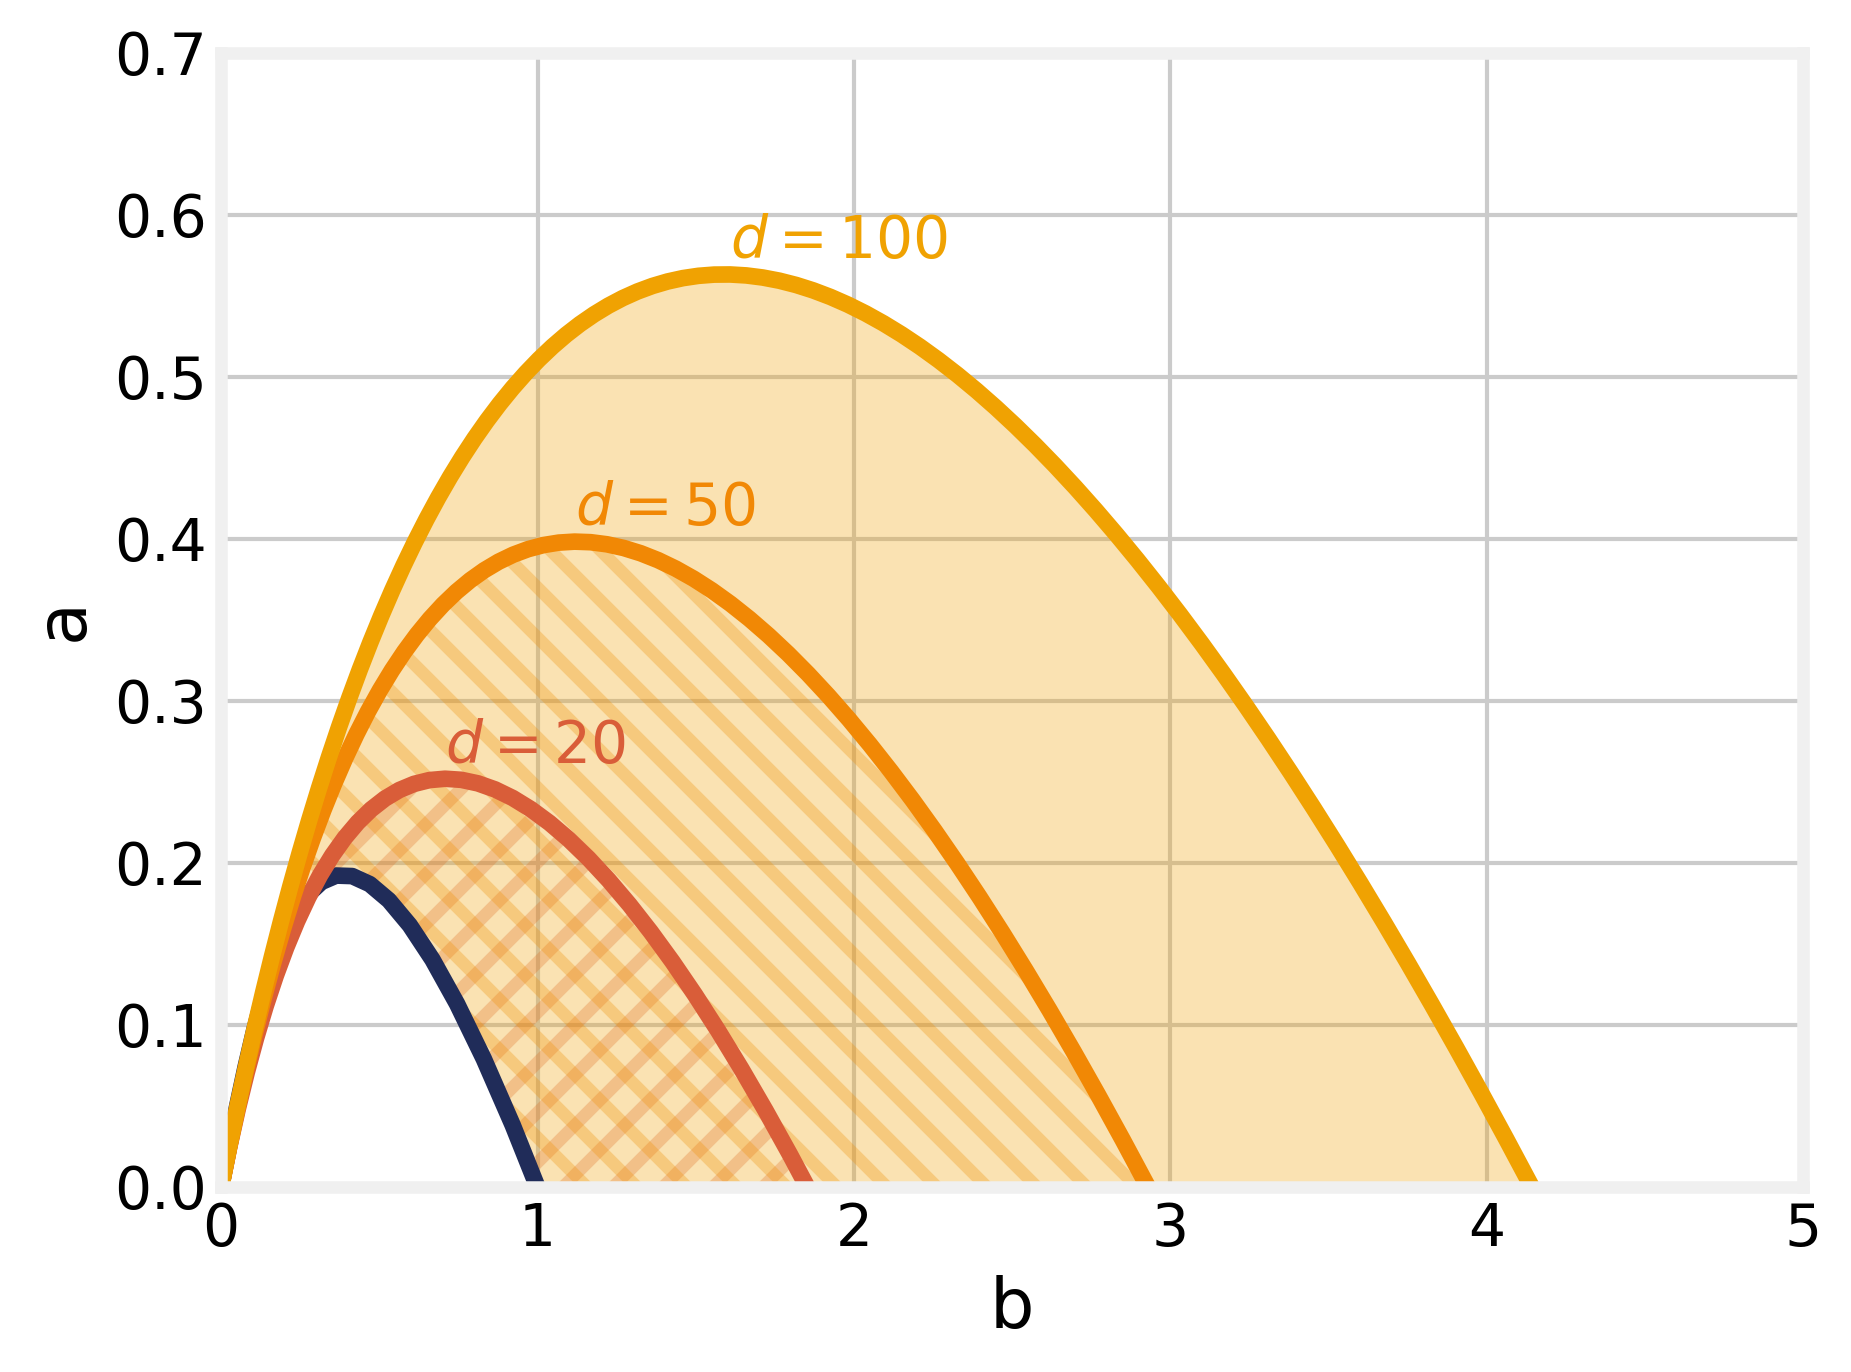
\includegraphics[width=0.5\linewidth]{img/Turing_space.png}
    \caption{The Turing space for \cref{eq:schnakenberg_reactions} plotted for $d = 20$, $d = 50$ and $d = 100$.}
    \label{fig:turingspace}
\end{figure}

\begin{figure}[htbp]
    \centering

    \begin{subfigure}{\textwidth}
        \centering
        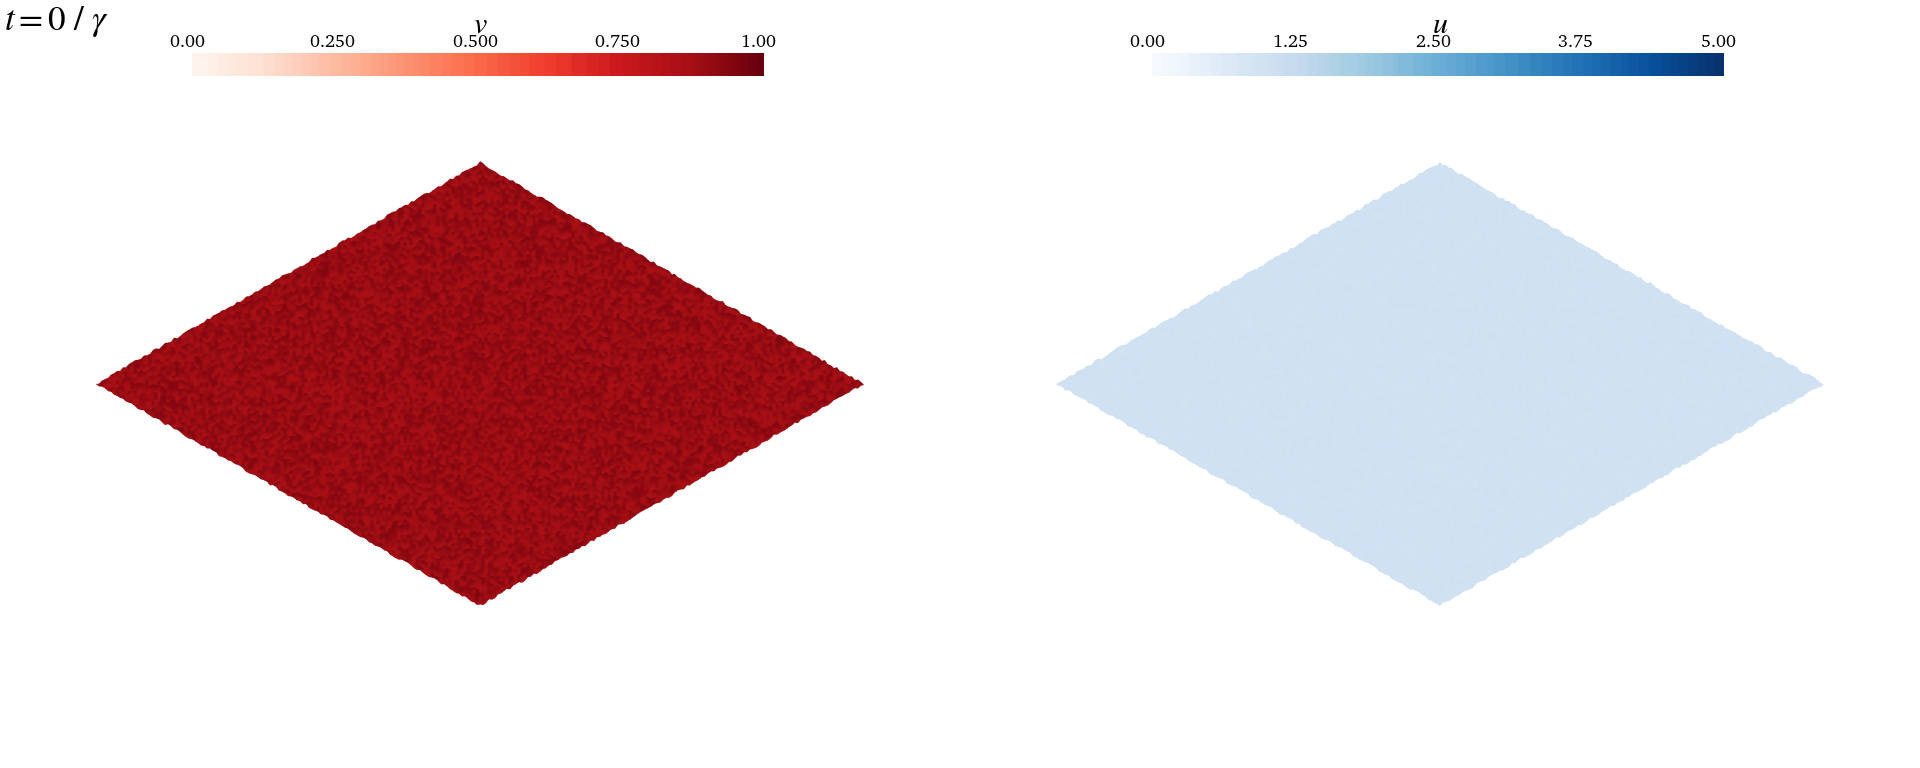
\includegraphics[width=\linewidth]{img/simulation_frames/schnakenberg_1.png}
        \caption{Caption 1}
    \end{subfigure}

    \vspace{0.4cm}

    \begin{subfigure}{\textwidth}
        \centering
        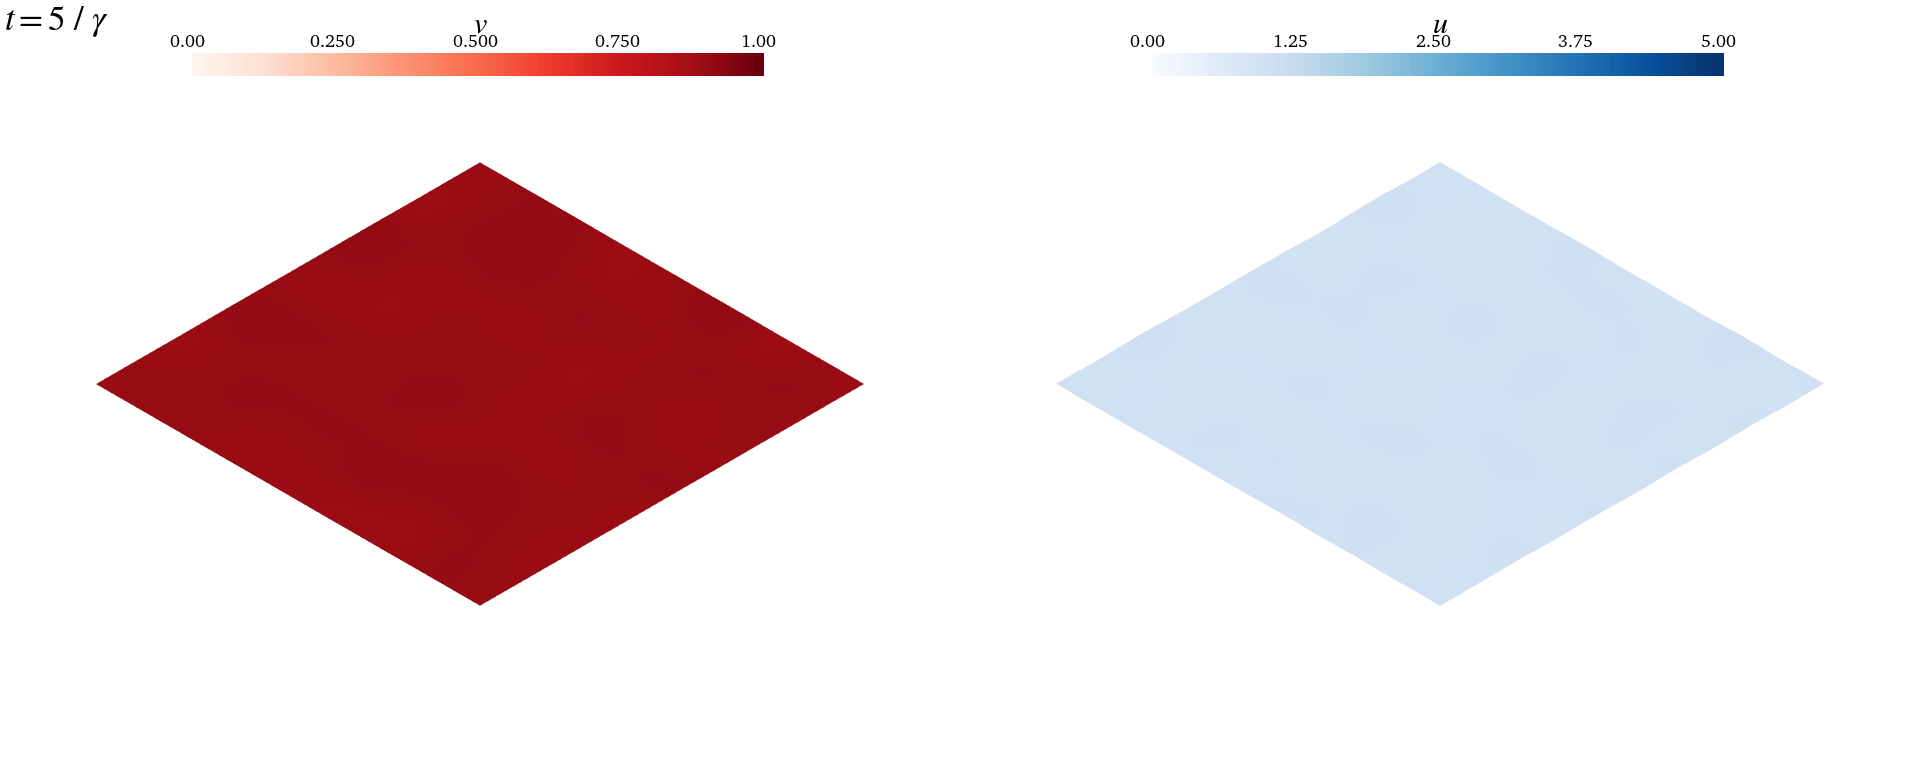
\includegraphics[width=\linewidth]{img/simulation_frames/schnakenberg_2.png}
        \caption{Caption 2}
    \end{subfigure}

    \vspace{0.4cm}

    \begin{subfigure}{\textwidth}
        \centering
        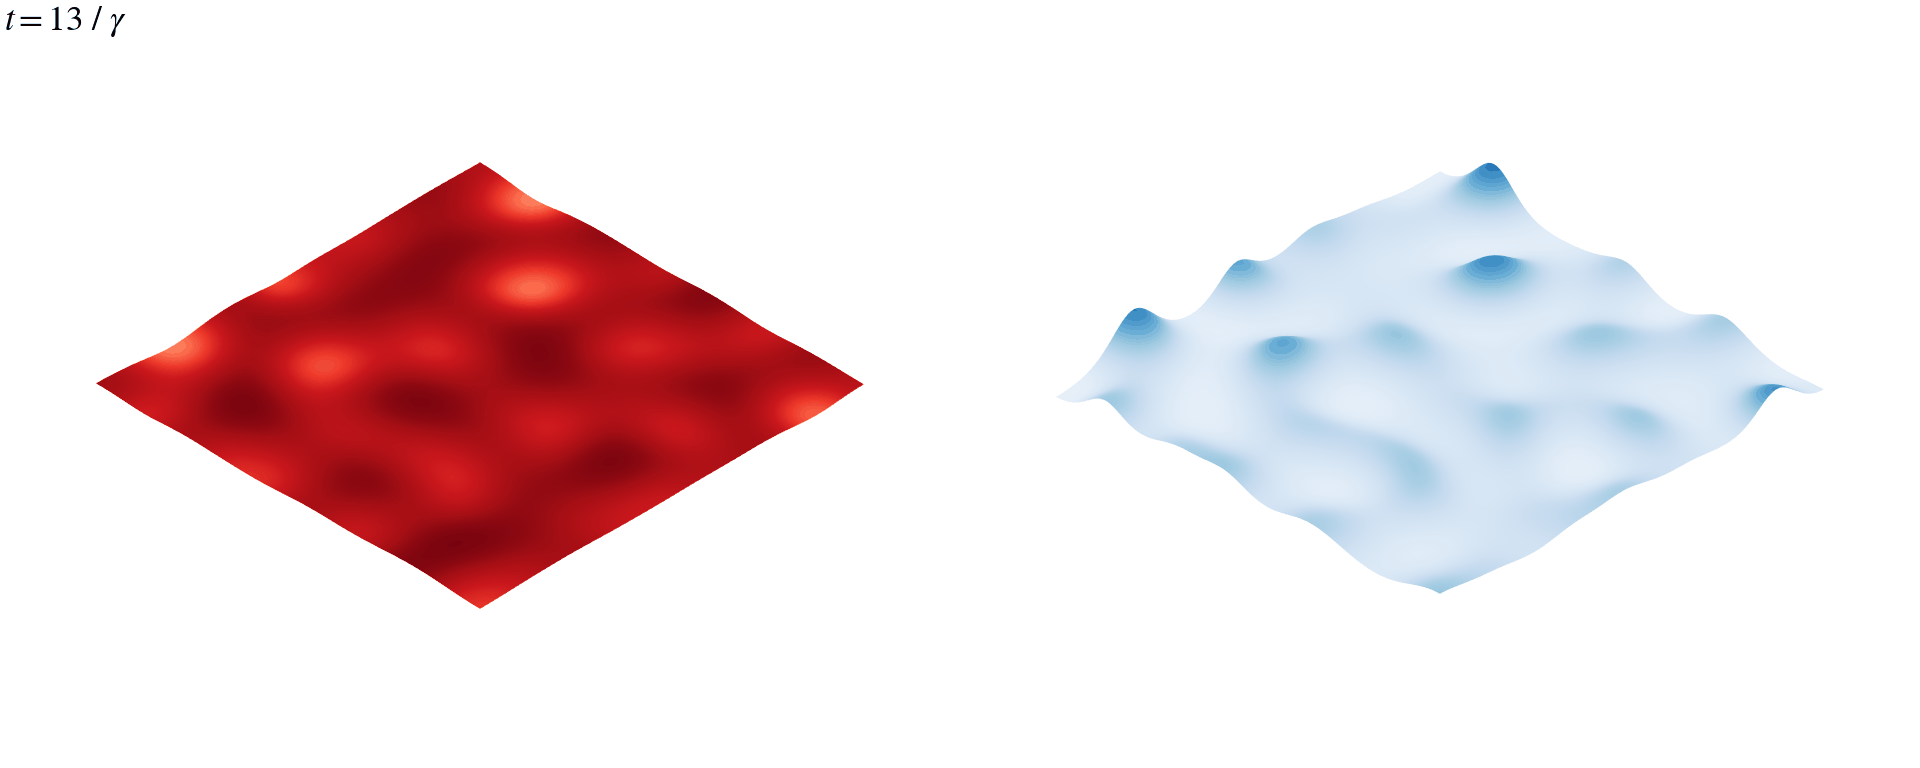
\includegraphics[width=\linewidth]{img/simulation_frames/schnakenberg_3.png}
        \caption{Caption 3}
    \end{subfigure}

    \caption{Overall figure caption.}
    \label{fig:schnakenberg_frames_1-3}
\end{figure}

\begin{figure}[htbp]
    \centering

    \begin{subfigure}{\textwidth}
        \centering
        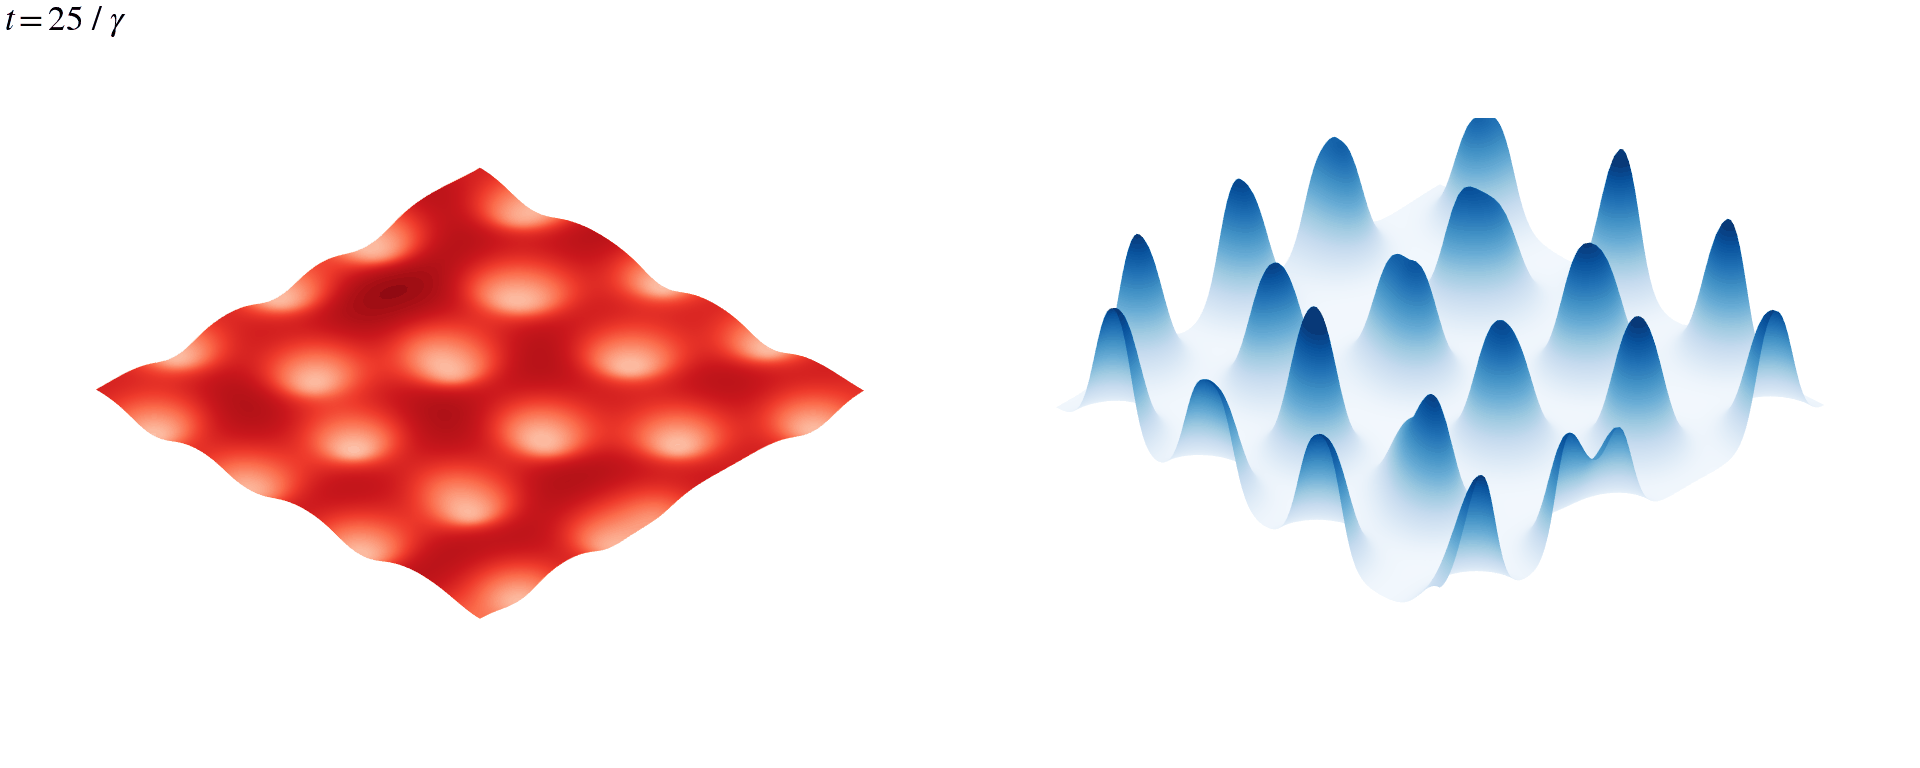
\includegraphics[width=\linewidth]{img/simulation_frames/schnakenberg_4.png}
        \caption{Caption 4}
    \end{subfigure}

    \vspace{0.4cm}

    \begin{subfigure}{\textwidth}
        \centering
        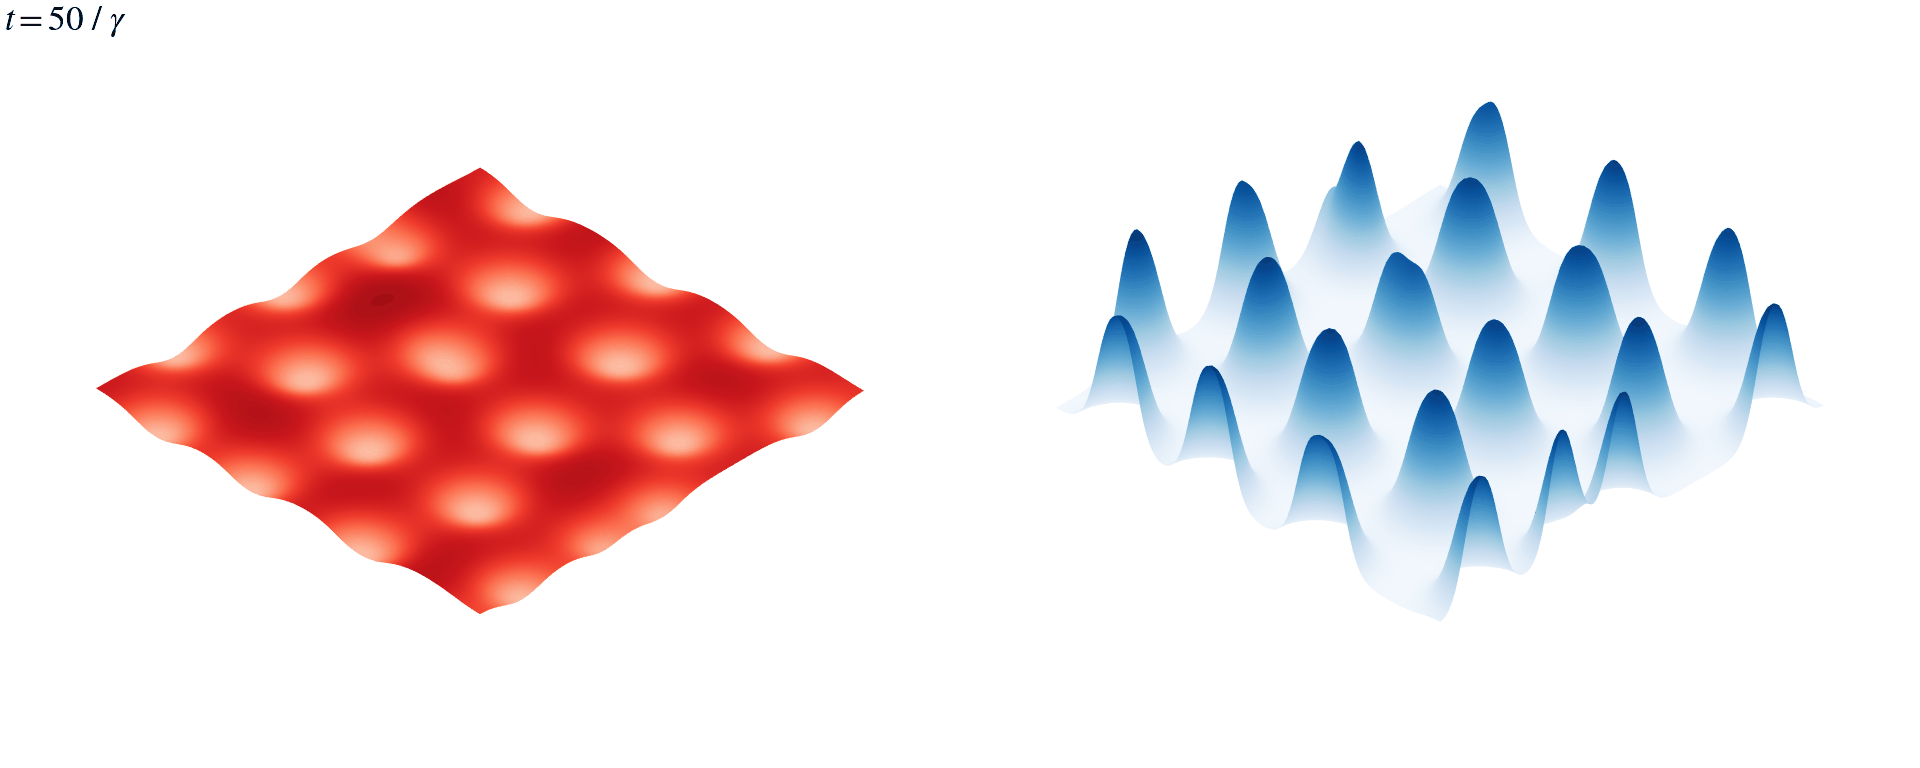
\includegraphics[width=\linewidth]{img/simulation_frames/schnakenberg_5.png}
        \caption{Caption 5}
    \end{subfigure}

    \vspace{0.4cm}

    \begin{subfigure}{\textwidth}
        \centering
        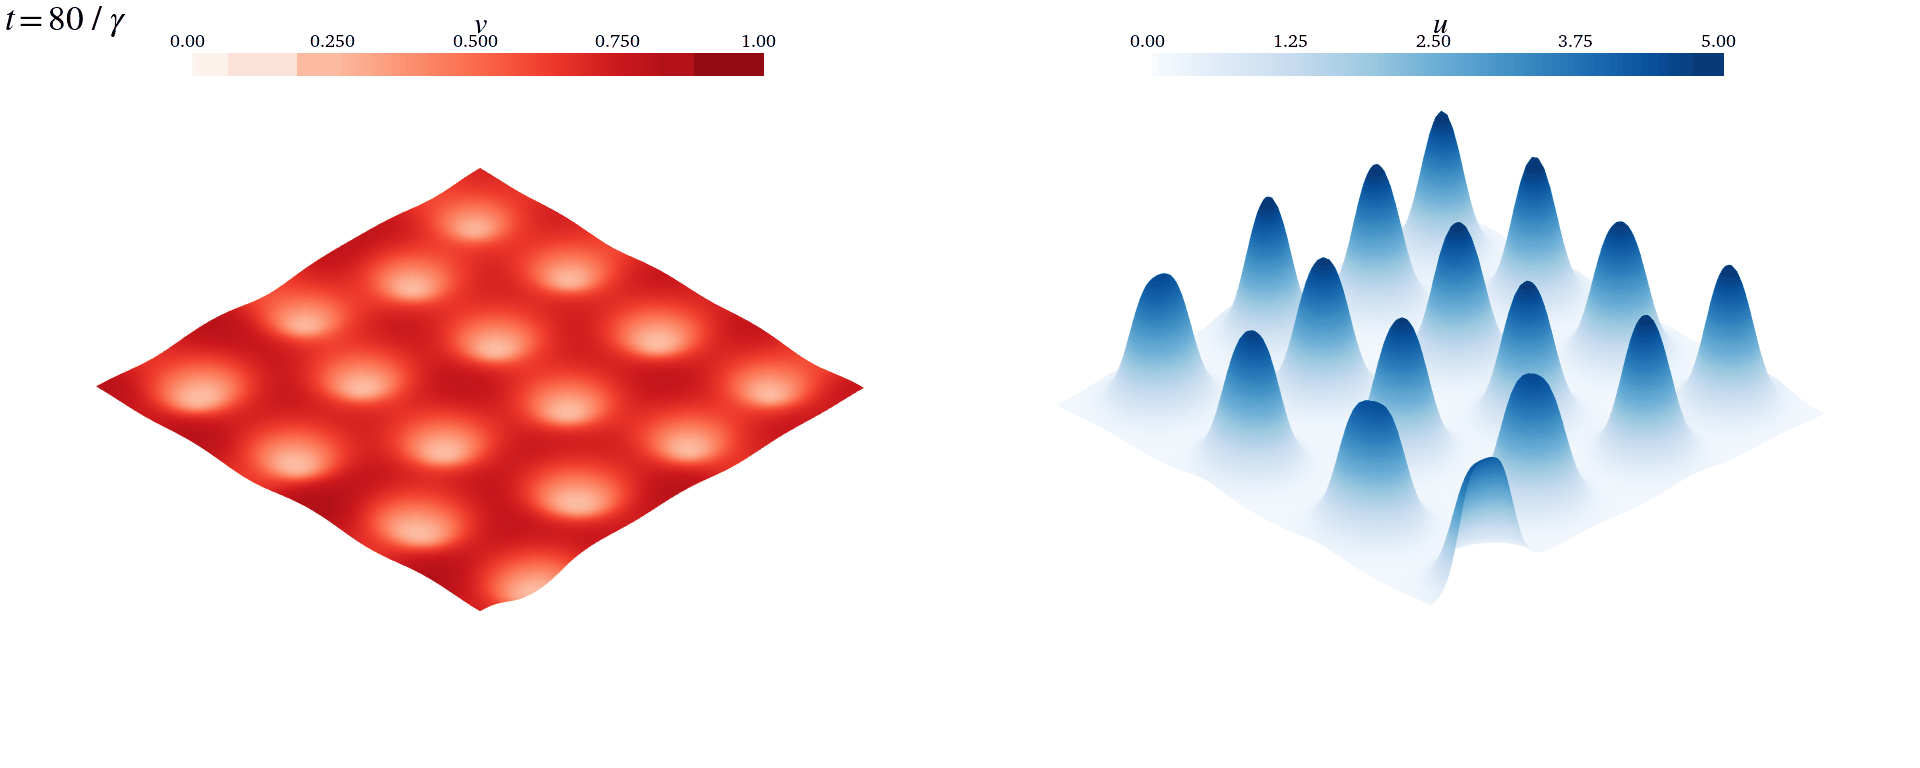
\includegraphics[width=\linewidth]{img/simulation_frames/schnakenberg_6.png}
        \caption{Caption 6}
    \end{subfigure}

    \caption{Overall figure caption.}
    \label{fig:schnakenberg_frames_4-6}
\end{figure}

\section{Example: Schnakenberg with decay}
\label{sec:schnakenberg_decay_example}
The $-u$ term in \cref{eq:schnakenberg_reactions} could be interpreted as natural decay of the species represented by $u$. We show that the addition of decay of $v$ does not cause the model to lose its ability to generate Turing patterns. To this end, consider the kinetics

\begin{equation}
    f(u, v) = a - u + u^2 v \qquad \text{and} \qquad g(u, v) = b - \delta_v v - u^2 v,
\end{equation}

\noindent
where $\delta_v > 0$ is the decay coefficient for $v$. When we use these new kinetics in the model of \cref{eq:reac_diff} with the new parameter $\delta_v$ set to $0.1$, we see from the simulations in \cref{fig:schnak_dec_1-3} are also able to generate Turing patterns. In this simulation, the other parameters are set to the same values as before, i.e. $d = 50$, $a = 0.1$, $b = 0.9$ and $\gamma = 8$. The domain is $\Omega = (-8, 8)^2$ again, and the initial conditions are the same as in \cref{eq:schnakenberg_initial} with

\begin{equation*}
    V := \frac{b}{U^2 + \delta_v}
\end{equation*}

\noindent
and $U$ being a positive real root of

\begin{equation*}
    U^3 - (a + b)U^2 + \delta_v U - a \delta_v = 0,
\end{equation*}

\noindent
if such a root exists. One can check that if $\delta_v = 0$, this returns the uniform steady states from the classical Schnakenberg equations, given in \cref{eq:schnakenberg_steadystates}.